\documentclass[10pt]{extarticle}
\title{}
\author{Avinash Iyer}
\date{}
\usepackage[shortlabels]{enumitem}


%paper setup
\usepackage{geometry}
\geometry{letterpaper, portrait, margin=1in}
\usepackage{fancyhdr}

%symbols
\usepackage{amsmath}
\usepackage{amssymb}
\usepackage{amsthm}
\usepackage{mathtools}
\usepackage{hyperref}
\usepackage{gensymb}
\usepackage{multirow,array}

\newtheorem*{remark}{Remark}
\usepackage[T1]{fontenc}
\usepackage[utf8]{inputenc}

%chemistry stuff
%\usepackage[version=4]{mhchem}
%\usepackage{chemfig}

%plotting
\usepackage{pgfplots}
\usepackage{tikz}
\tikzset{middleweight/.style={pos = 0.5, fill=white}}
\tikzset{weight/.style={pos = 0.5, fill = white}}
\tikzset{lateweight/.style={pos = 0.75, fill = white}}
\tikzset{earlyweight/.style={pos = 0.25, fill=white}}

%\usepackage{natbib}

%graphics stuff
\usepackage{graphicx}
\graphicspath{ {./images/} }
\usepackage[style=numeric, backend=biber]{biblatex} % Use the numeric style for Vancouver
\addbibresource{the_bibliography.bib}
%code stuff
%when using minted, make sure to add the -shell-escape flag
%you can use lstlisting if you don't want to use minted
%\usepackage{minted}
%\usemintedstyle{pastie}
%\newminted[javacode]{java}{frame=lines,framesep=2mm,linenos=true,fontsize=\footnotesize,tabsize=3,autogobble,}
%\newminted[cppcode]{cpp}{frame=lines,framesep=2mm,linenos=true,fontsize=\footnotesize,tabsize=3,autogobble,}

%\usepackage{listings}
%\usepackage{color}
%\definecolor{dkgreen}{rgb}{0,0.6,0}
%\definecolor{gray}{rgb}{0.5,0.5,0.5}
%\definecolor{mauve}{rgb}{0.58,0,0.82}
%
%\lstset{frame=tb,
%	language=Java,
%	aboveskip=3mm,
%	belowskip=3mm,
%	showstringspaces=false,
%	columns=flexible,
%	basicstyle={\small\ttfamily},
%	numbers=none,
%	numberstyle=\tiny\color{gray},
%	keywordstyle=\color{blue},
%	commentstyle=\color{dkgreen},
%	stringstyle=\color{mauve},
%	breaklines=true,
%	breakatwhitespace=true,
%	tabsize=3
%}
% text + color boxes
\usepackage[most]{tcolorbox}
\tcbuselibrary{breakable}
\newtcolorbox{problem}[1]{colback = white, title = {#1}, breakable}
\newtcolorbox{solution}{colback = white, colframe = black!75!white, title = Solution, breakable}
%including PDFs
%\usepackage{pdfpages}
\setlength{\parindent}{0pt}
\usepackage{cancel}
\pagestyle{fancy}
\fancyhf{}
\rhead{Avinash Iyer}
\lhead{}
\newcommand{\card}{\text{card}}
\newcommand{\ran}{\text{ran}}
\newcommand{\N}{\mathbb{N}}
\newcommand{\Q}{\mathbb{Q}}
\newcommand{\Z}{\mathbb{Z}}
\newcommand{\R}{\mathbb{R}}
\begin{document}
  \begin{problem}{Charter Evidence}
    Abdulkadiroglu et al. (2011) studied the effectiveness of charter schools in the Boston area using a clever research strategy. They utilized the fact that many charter schools in the area are oversubscribed, and thus must assign enrollment slots to students using a randomized lottery. The researchers compared winners and losers of the lottery to estimate the effect of charter school attendance on student achievement, finding large and significant score gains for charter students compared to their peers who lost the lottery.\\

    Based on the results of this experiment, one policy maker has argued that all schools in the state of Massachusetts should be replaced by charter schools. In what ways does the experiment support this policymaker's proposal? Now, considering the other side of the debate, what are \textit{two} specific reasons for proceeding with caution when applying the results of the experiment to this proposal?
    \tcblower
    The experiment does support the proposal insofar as it shows sizable improvements for students who go to charter schools compared to those who go to public schools \textit{among the group of people who would go to charter schools otherwise}.\\

    However, there are two specific problems with the proposed policy
    \begin{enumerate}[(a)]
      \item Families choosing charter schools may not have the requisite information to choose a school that best serves their child.
      \item Charter-izing all of the schools could yield lower average quality of charter schools compared to the current model, muting their benefits as they currently stand.
    \end{enumerate}
  \end{problem}
  \begin{problem}{Voucher Effects}
    The town of Greenville has three families, each with one child, each of which earns \$20,000 per year (pre-tax). The three families, $X$, $Y$, and $Z$ differ in their preferences for education, with corresponding utility functions over education $E$ and consumption $C$ as follows:
    \begin{align*}
      U_X(E,C) &= 0.25\ln(E) + 0.75\ln(C)\\
      U_Y(E,C) &= 0.5\ln(E) + 0.5\ln(C)\\
      U_Z(E,C) &= 0.75\ln(E) + 0.25\ln(C)
    \end{align*}
    Let the unit prices of $E$ and $C$ be normalized to \$1.\\

    Consider the following public education finance policy. Each family is taxed \$4,000 per year to finance the public school system in the town, which any family can then freely attend. Education spending is \$6,000 per student in the public schools. The only way a family can choose more than \$6,000 in education spending is by sending their child to private school. The budget constraint for each family is the line $LMNO$ below.
    \begin{center}
      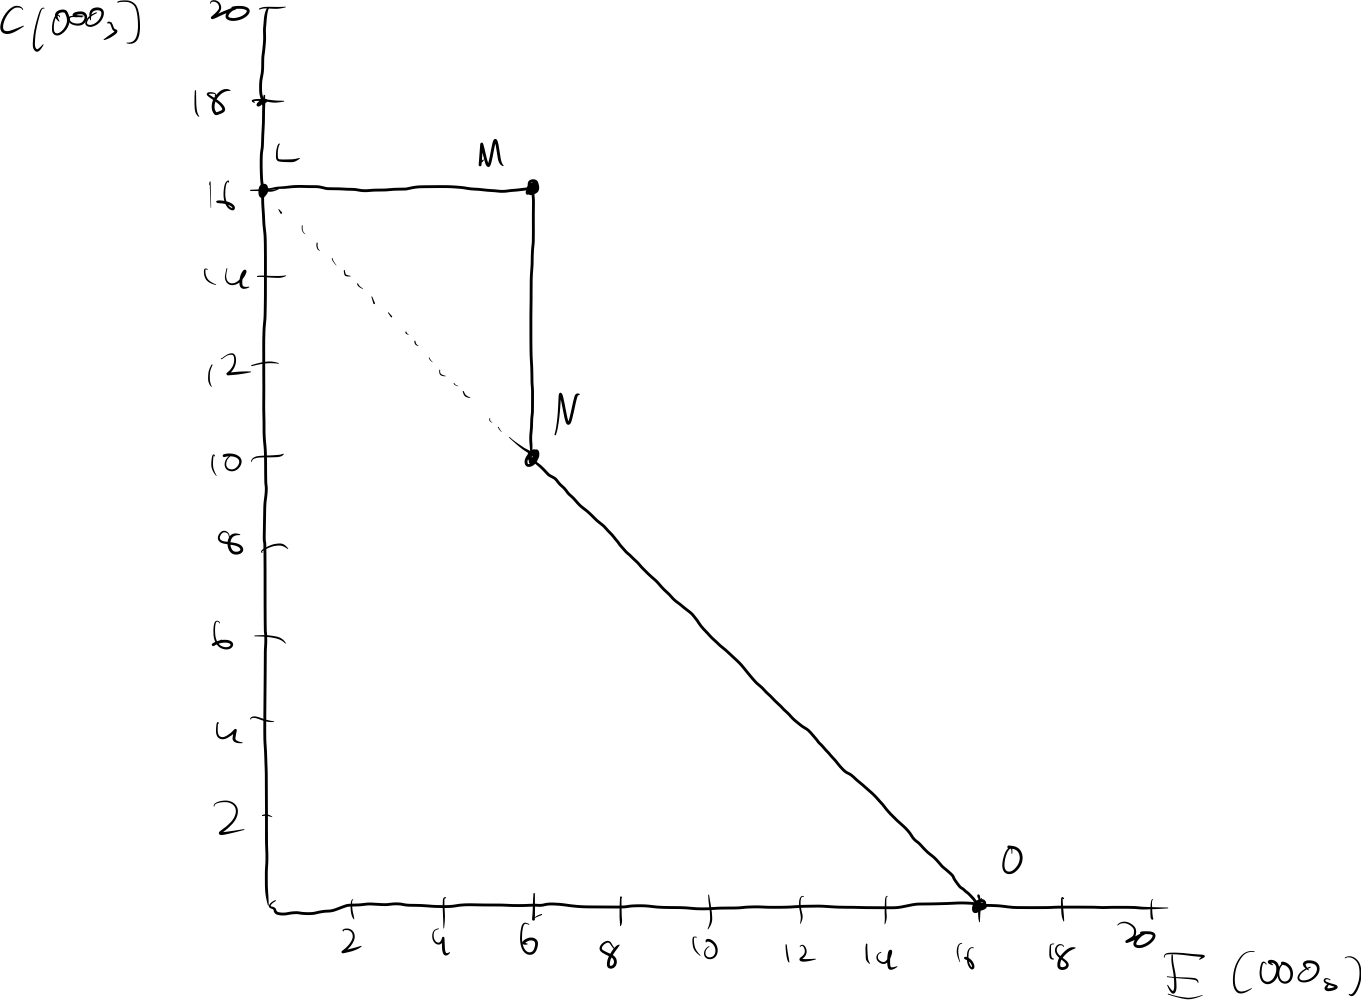
\includegraphics[width=10cm]{4_2}
    \end{center}
    \tcblower
    \begin{problem}{(a)}
      Determine the utility-maximizing choices for each family.
      \tcblower
      \begin{description}[font=\normalfont]
        \item[Family $X$:] $E = 6,000,~C = 16,000$
        \item[Family $Y$:] $E = 8,000,~C=8,000$
        \item[Family $Z$:] $E = 12,000,~C=4,000$
      \end{description}
    \end{problem}
    \begin{problem}{(b)}
      In the figure above, draw corresponding indifference curves for each family at their utility-maximizing choices in part (a).
      \tcblower
      \begin{center}
        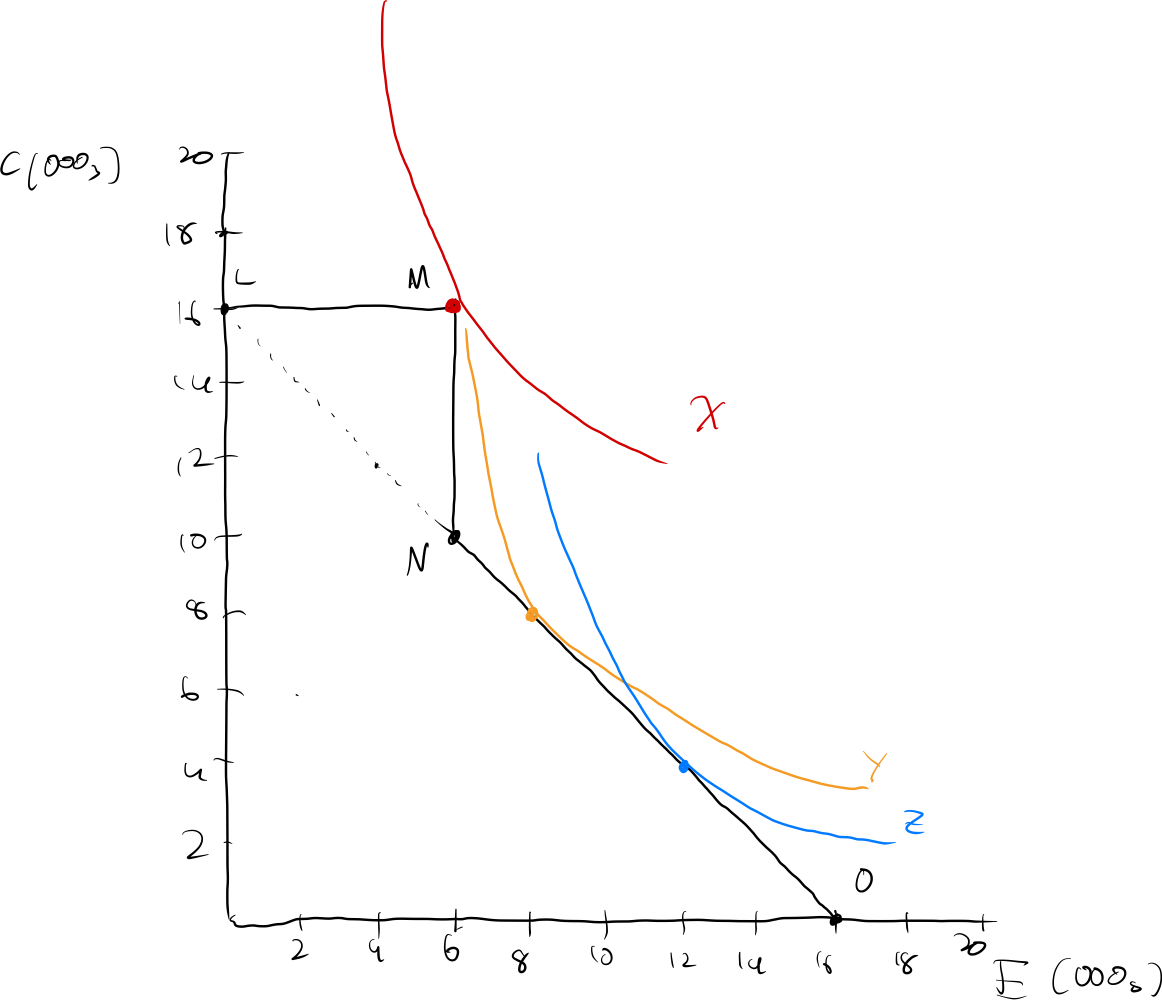
\includegraphics[width=10cm]{4_2_b}
      \end{center}
    \end{problem}
    \begin{problem}{(c)}
      Which families use the public school system and which send their child to the private school?
      \tcblower
      Family $X$ sends their child to public school, and families $Y$ and $Z$ send their child to private school.
    \end{problem}
    The town is considering replacing its current system with a voucher system. Under the new system, each family would receive a \$6,000 voucher for education, and families would still be able to send their children to the public school. Since this would be more costly than the current system, they would also raise taxes to \$6,000 per household to pay for it. The budget constraint for each family is now the $QRS$.
    \begin{center}
      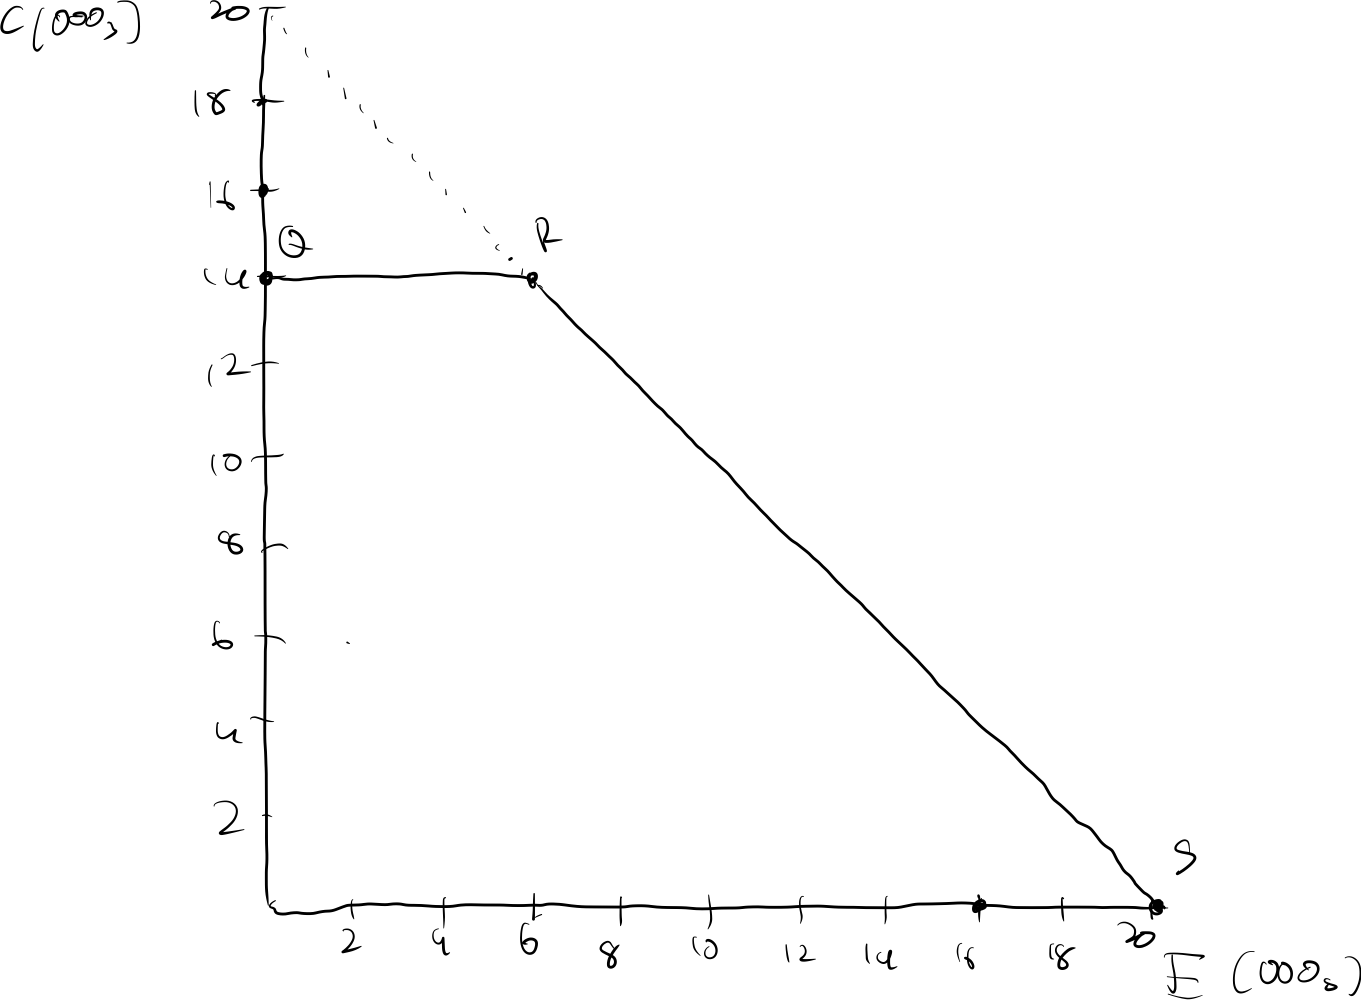
\includegraphics[width=10cm]{4_2_1}
    \end{center}
    \begin{problem}{(d)}
      Determine the utility-maximizing choices for each family with this voucher policy.
      \tcblower
      \begin{description}[font=\normalfont]
        \item[Family $X$:] $E = 6,000$, $C = 14,000$
        \item[Family $Y$:] $E = 10,000$, $C = 10,000$
        \item[Family $Z$:] $E = 15,000$, $C = 5,000$
      \end{description}
    \end{problem}
    \begin{problem}{(e)}
      Draw the corresponding indifference curves for each family at their utility-maximizing choices in part (d).
      \tcblower
      \begin{center}
        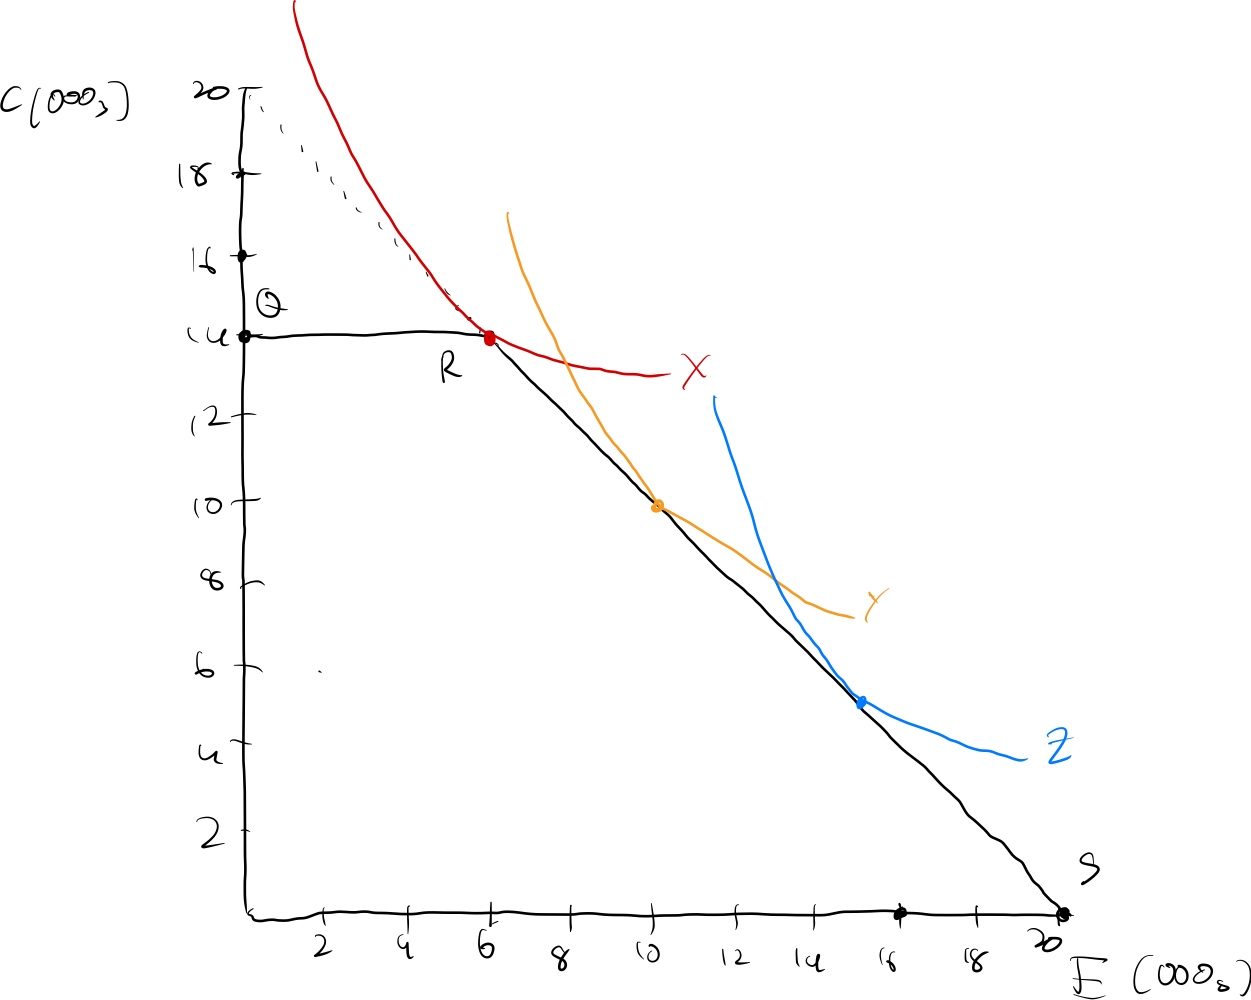
\includegraphics[width=10cm]{4_2_d}
      \end{center}
    \end{problem}
    \begin{problem}{(f)}
      Now which families use the public school system and which send their child to private school?
      \tcblower
      The effect on each family is the same --- no family switches from public to private school or vice versa.
    \end{problem}
    \begin{problem}{(g)}
      Which families are made better off and which families are made worse off by the voucher policy?
      \tcblower
      Family $X$ is made worse off, and families $Y$ and $Z$ are made better off.
    \end{problem}
  \end{problem}
  \begin{problem}{Modeling Intergenerational Mobility}
    Consider a discrete-time setting in which $t$ indexes generations. For simplicity, assume that each family, indexed by $i$, consists of a single individual in each generation $t$. Let $y_{i,t}$ denote the income percentile rank of individual $i$ relative to all other individuals in the same generation $t$, and let $r$ denote the race of family $i$. Consistent with empirical evidence, let's model individual $i$'s income rank as a race-specific linear function of their parents' income rank:
    \begin{equation}
      y_{i,t} = \alpha_r + \beta_r y_{i,t-1}
    \end{equation}
    where $\alpha_r$ and $\beta_r$ are race-specific parameters between zero and one.
    \begin{problem}{(a)}
      Provide an interpretation of $\alpha_r$.
      \tcblower
      $\alpha_r$ is the average income percentile of the current generation of people whose parents were at income percentile $0$ in the previous generation.
    \end{problem}
    \begin{problem}{(b)}
      In a society for which parents' incomes matter very little for the incomes of their children, is $\beta_r$ large or small?
      \tcblower
      $\beta_r$ would be small --- i.e., the effect of $y_{i,t-1}$ on $y_{i,t}$ would also be very small.
    \end{problem}
    Assume that $\alpha_b = 0.25$ and $\beta_b = 0.29$ for blacks, while $\alpha_w = 0.37$ and $\beta_w = 0.32$ for whites.
    \begin{problem}{(c)}
      Consider two families, one Black and one white, each in the 10th percentile of the income distribution for the current generation. Use the model and parameters to predict the income percentile rank for each family's grandchildren.
      \tcblower
      For the Black family, $y_{i,t+2}$ would be at the 33rd percentile, while for the White family, $y_{i,t+2}$ would be at the 50th percentile.
    \end{problem}
    \begin{problem}{(d)}
      Repeat part (c), but for two families in the 90th percentile of the current income distribution.
      \tcblower
      For the Black family, $y_{i,t+2} = 0.398$, while for the white family, $y_{i,t+2} = 0.581$
    \end{problem}
    Let $\overline{y}_{r,t}$ indicate the mean rank of individuals of race $r$ in generation $t$. Then, it follows from equation (1) that:
    \begin{equation}
      \overline{y}_{r,t} = \alpha_r + \beta_r \overline{y}_{r,t-1}
    \end{equation}
    Define the steady state mean rank of race $r$, denoted by $\overline{y}_r^{SS}$, as the mean rank of race $r$ for which there is no generational change.
    \begin{problem}{(e)}
      Determine $\overline{y}_b^{SS}$ and $\overline{y}_{w}^{SS}$.
      \tcblower
      \begin{align*}
        \overline{y}_b^{SS} &= 0.352\\
        \overline{y}_w^{SS} &= 0.544
      \end{align*}
    \end{problem}
    \begin{problem}{(f)}
      How do your answers in part (e) compare to your answers in part (c) and (d). Interpret.
      \tcblower
      The steady states for Black and white families are attractive fixed points of the $\overline{y}_{r,t}$, meaning that the steady state is higher than the answers for part (c) and lower than those for part (d).
    \end{problem}
    Answer the following questions based on the evidence presented by Raj Chetty for observed mean ranks and predicted steady-state mean ranks across five race categories: American Indian, Asian, Black, Hispanic, and white.
    \begin{problem}{(g)}
      Which race category has seen the largest increase in mean rank from parents to their children born int he early 1980s?
      \tcblower
      Hispanics have seen the largest increase.
    \end{problem}
    \begin{problem}{(h)}
      Which race category has seen the largest decrease in mean rank from parents to their children born in the early 1980s?
      \tcblower
      Asians have seen the largest decrease.
    \end{problem}
    \begin{problem}{(i)}
      Which race category appears closest to its predicted steady state?
      \tcblower
      American Indians are closest to their predicted steady state.
    \end{problem}
  \end{problem}
  \begin{problem}{Moving to Opportunity}
    \begin{problem}{(a)}
      The Moving to Opportunity experiment was implemented in the Clinton administration, by the Housing and Urban Development agency, from 1994 to 1998 in five major cities in the United States: Baltimore, Boston, Chicago, L.A., and New York. HUD randomly assigned 4,600 families to three different groups. The experimental group was offered a housing voucher that required them to move to a low-poverty census tract (less than 10\% poverty rate). The Section 8 voucher group was offered the same value of housing voucher but with no restrictions. The control group was not offered a voucher. Inspect and interpret the evidence from this RCT.
      \tcblower
      It appears that Moving to Opportunity has a much stronger positive effect on children under 13, while it has little or even a negative effect on children above 13.
    \end{problem}
    \begin{problem}{(b)}
      In the given figure each dot represents a different census tract of a different neighborhood in Seattle. Interpret the slope of the best fit line through the data. And which quadrant of the plot identifies potential ``opportunity bargains'' --- affordable options with high mobility.
      \tcblower
      The slope of the graph implies that places with higher 2 bedroom rents tend to also have higher incomes for children of low-income parents. However, this does imply that places in the top left of the graph (with relatively low 2 bedroom rents and high incomes for children of low-income parents) are an opportunity bargain.
    \end{problem}
    \begin{problem}{(c)}
      The participants in the Creating Moves to Opportunity (CMTO) experiment in Seattle were restricted to families eligible to receive a housing voucher with young children. They were randomly assigned to a control or treatment group. The treatment group received information on which neighborhoods might provide better opportunities for their children, but were not required to move to a high opportunity area. They also received rental application assistance and housing locator services. The effect of the RCT is seen in the given figure.\\

      CMTO primarily shifted where families chose to live rather than whether families were able to use their voucher. 86\% of families in the control group leased a unit somewhere using their housing vouchers and 87\% of households in the treatment group leased a unit using a housing voucher. What does this evidence suggest about the factors that do and do not matter for whether people move to high-opportunity neighborhoods.
      \tcblower
      People tend to move to high opportunity neighborhoods when they receive information on it --- for example, the treatment effect appears to be 37.9 percentage points in favor of moving to opportunity upon receiving information. However, in spite of this, it does also appear that there is a substantial overlap between people who used their vouchers in high-opportunity areas and those who did not.
    \end{problem}
    \begin{problem}{(d)}
      Explain at least one concern/drawback/limitation with the CMTO as a policy approach.
      \tcblower
      CMTO may work on the margin, but a large scale ramping up of the program may mute its effects.
    \end{problem}
  \end{problem}
\end{document}
